\documentclass[a4paper,12pt]{article}

\usepackage{graphicx} % Required for inserting images
\usepackage{amsmath,amssymb,amsfonts}
\usepackage{subcaption}
% Use Times New Roman font
\usepackage{times}
\usepackage[a4paper, top=1in, bottom=0.8in, left=1.1in, right=0.8in]{geometry}
\usepackage{float}
\usepackage{listings}
\usepackage{xcolor} % For customizing code colors
\setlength{\parindent}{0pt}
\usepackage{titlesec} % Add this to your preamble
\titleformat{\section}
{\normalfont\large\bfseries}{\thesection}{1em}{}
% Set spacing for sections
\titlespacing*{\section}
{0pt}  % Left spacing
{1ex} % Space before (adjust this value)
{0ex}  % Space after (adjust this value)
\begin{document}
	\section{Experiment No. 5}
	
	
	\section{Experiment Title }
Design and analyze a 2 input NAND \& NOR  gate using nMOS inverter 
with Enhancement \& Resistive Load using 	MICROWIND 3.0
	\section{Objective}
	The main objectives of this report are:
	
	\begin{itemize}
		\item To design and analyze 2-input NAND and NOR gates using nMOS inverters with resistive and enhancement mode loads.
		\item To evaluate the performance of resistive and enhancement mode loads in terms of output voltage levels characteristics.
		\item To simulate and verify the logical behavior of NAND and NOR gates using MICROWIND 3.0 software.
	
	\end{itemize}
	\section{Theory}
	\subsection{nMOS Inverter with Enhancement Mode (Pull-Up) Load}


An nMOS inverter with an enhancement mode (pull-up) load consists of two nMOS transistors: the driving transistor (\(T_1\)) and the load transistor (\(T_2\)). The load transistor \(T_2\) is connected between the power supply \(V_{DD}\) and the output node, while \(T_1\) is connected between the output and ground. The gate of \(T_2\) is connected to \(V_{DD}\) to keep it ON when both inputs are low.\\
\begin{figure}[H]
	\centering
	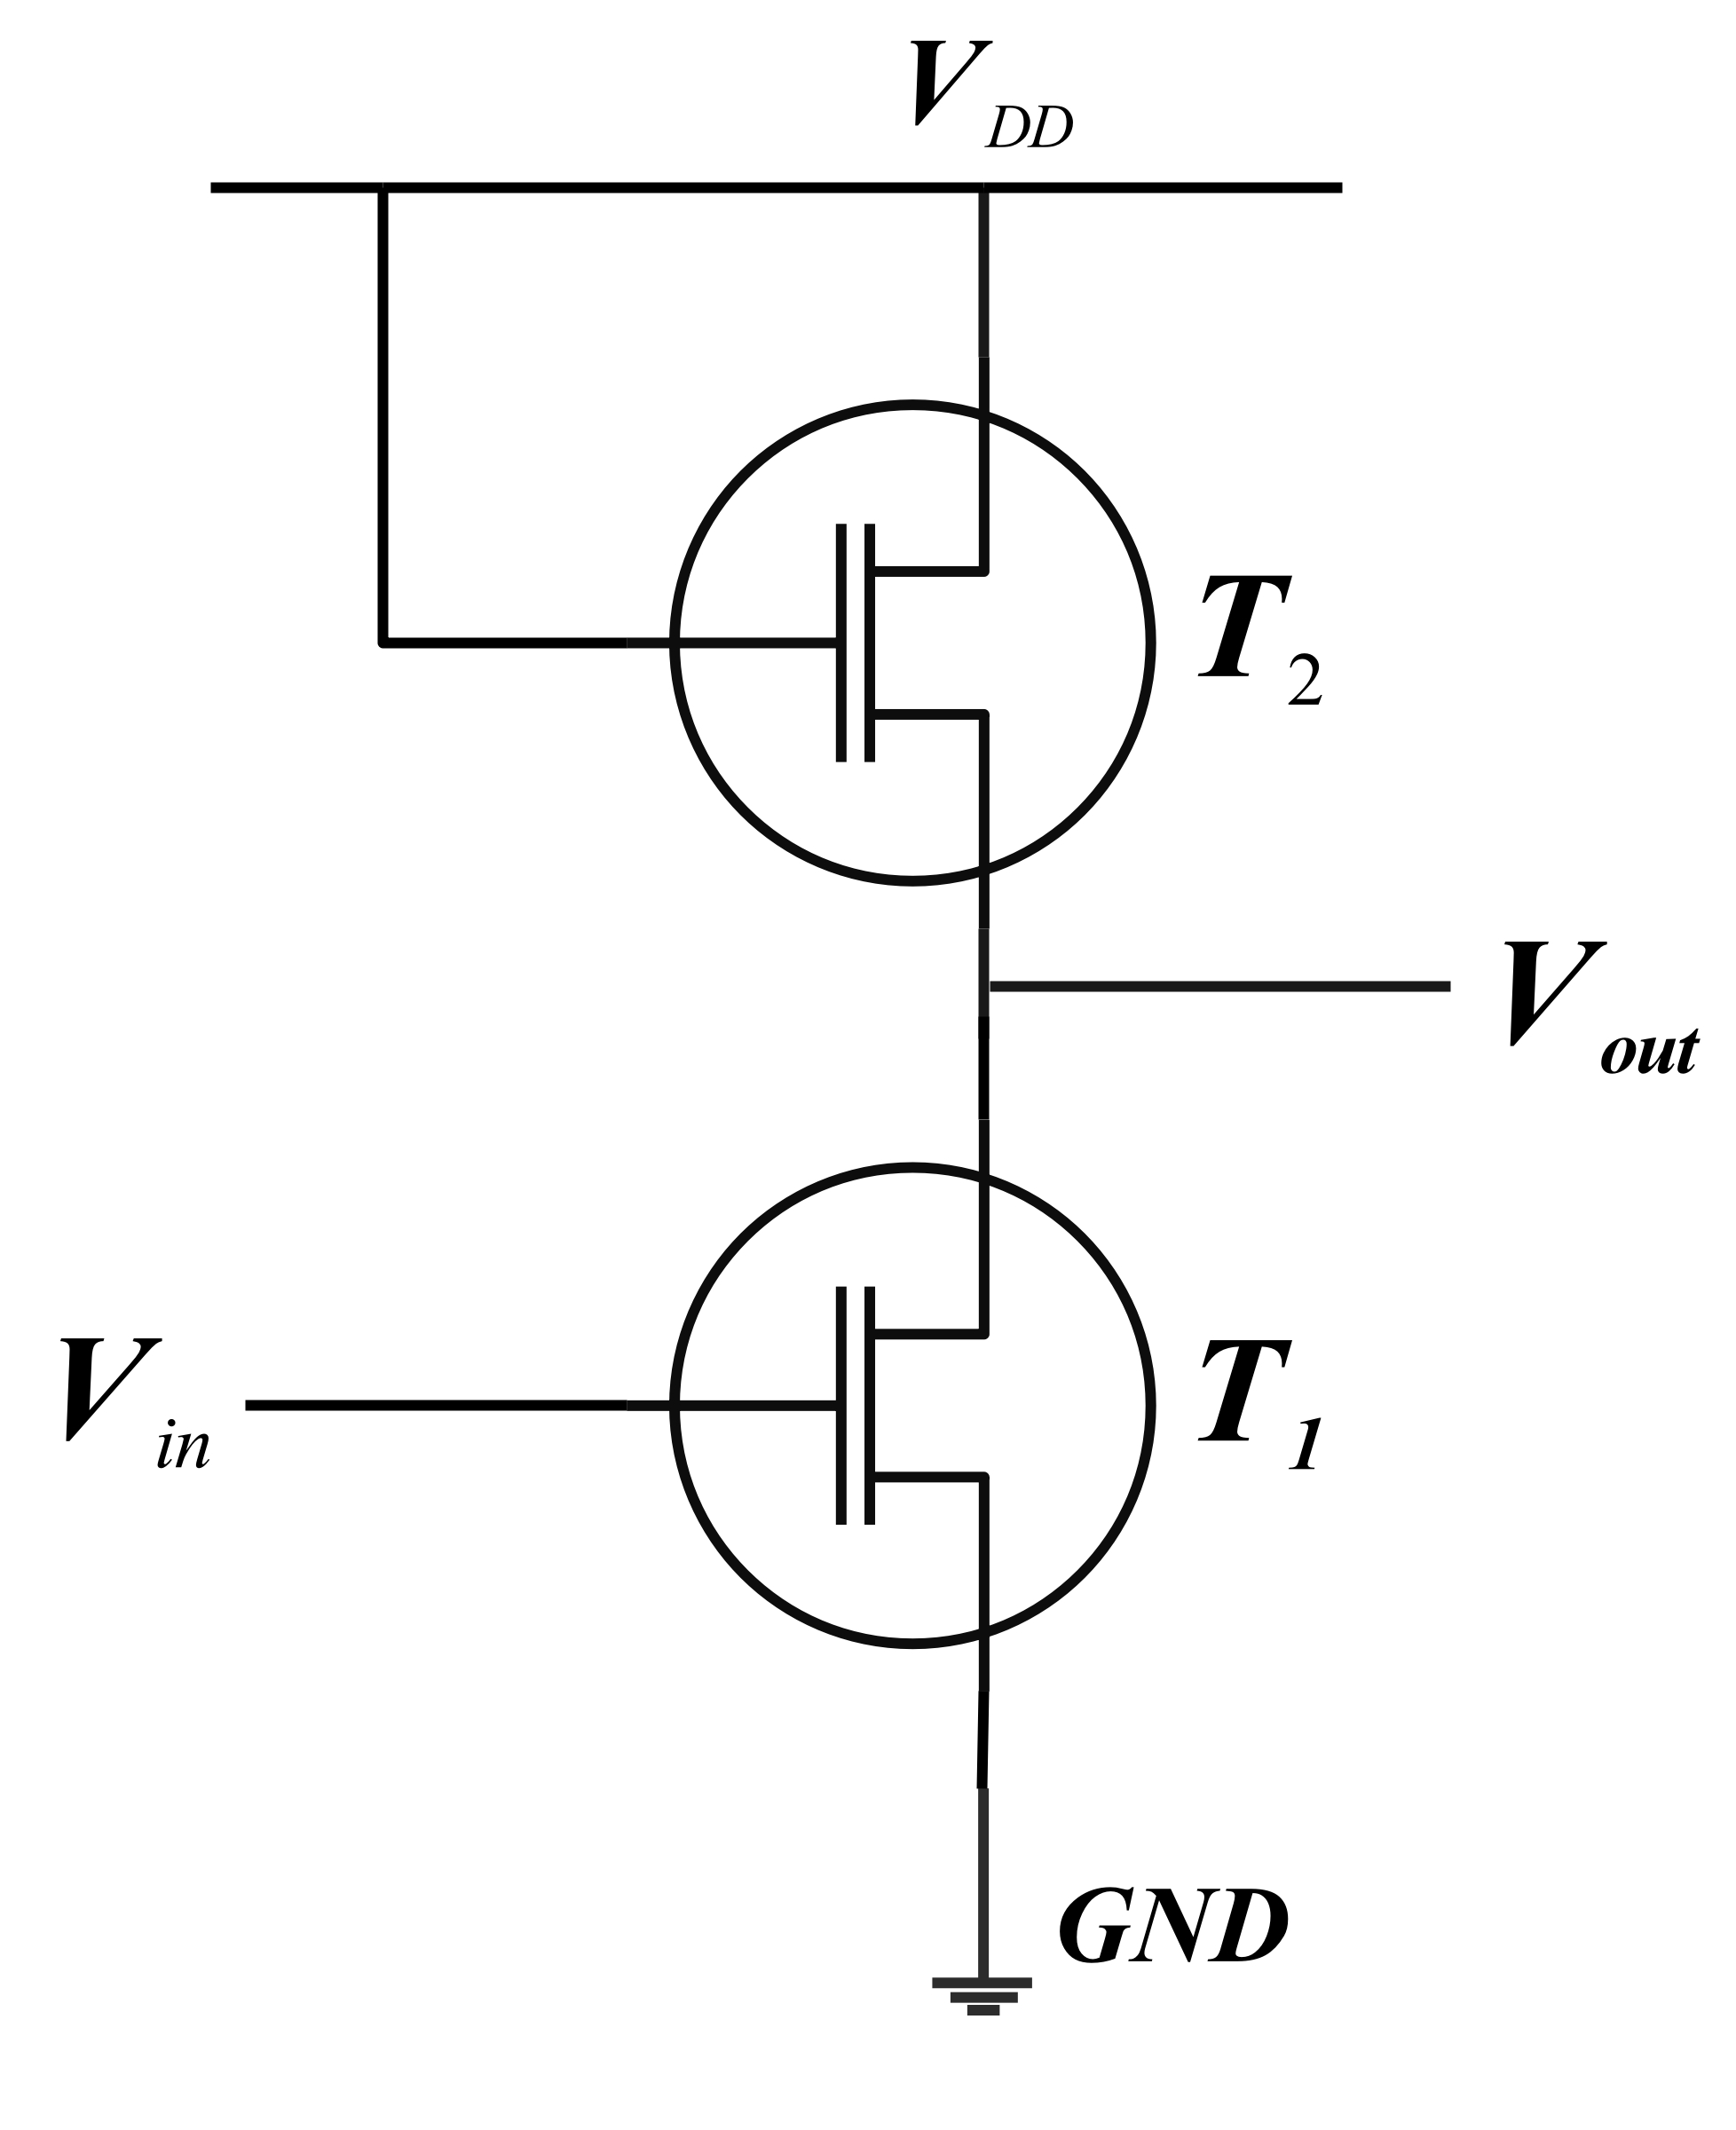
\includegraphics[width=0.45\linewidth]{../EXP04_EEE2214/Images/mos/1}
	\caption{}
	\label{fig:1}
\end{figure}

- When the input \(V_{in}\) is low (logic '0'), \(T_1\) is OFF, and \(T_2\) pulls the output \(V_{out}\) high to \(V_{DD}\).\\
- When \(V_{in}\) is high (logic '1'), \(T_1\) turns ON, pulling \(V_{out}\) low to 0V.


\subsection{nMOS Inverter with Resistive Load}

An nMOS inverter with a resistive load consists of an nMOS transistor (\(T_1\)) and a resistor (\(R_L\)). The resistor is connected between the power supply \(V_{DD}\) and the output node, while \(T_1\) is connected between the output and ground. The operation can be summarized as follows:
\begin{figure}[H]
	\centering
	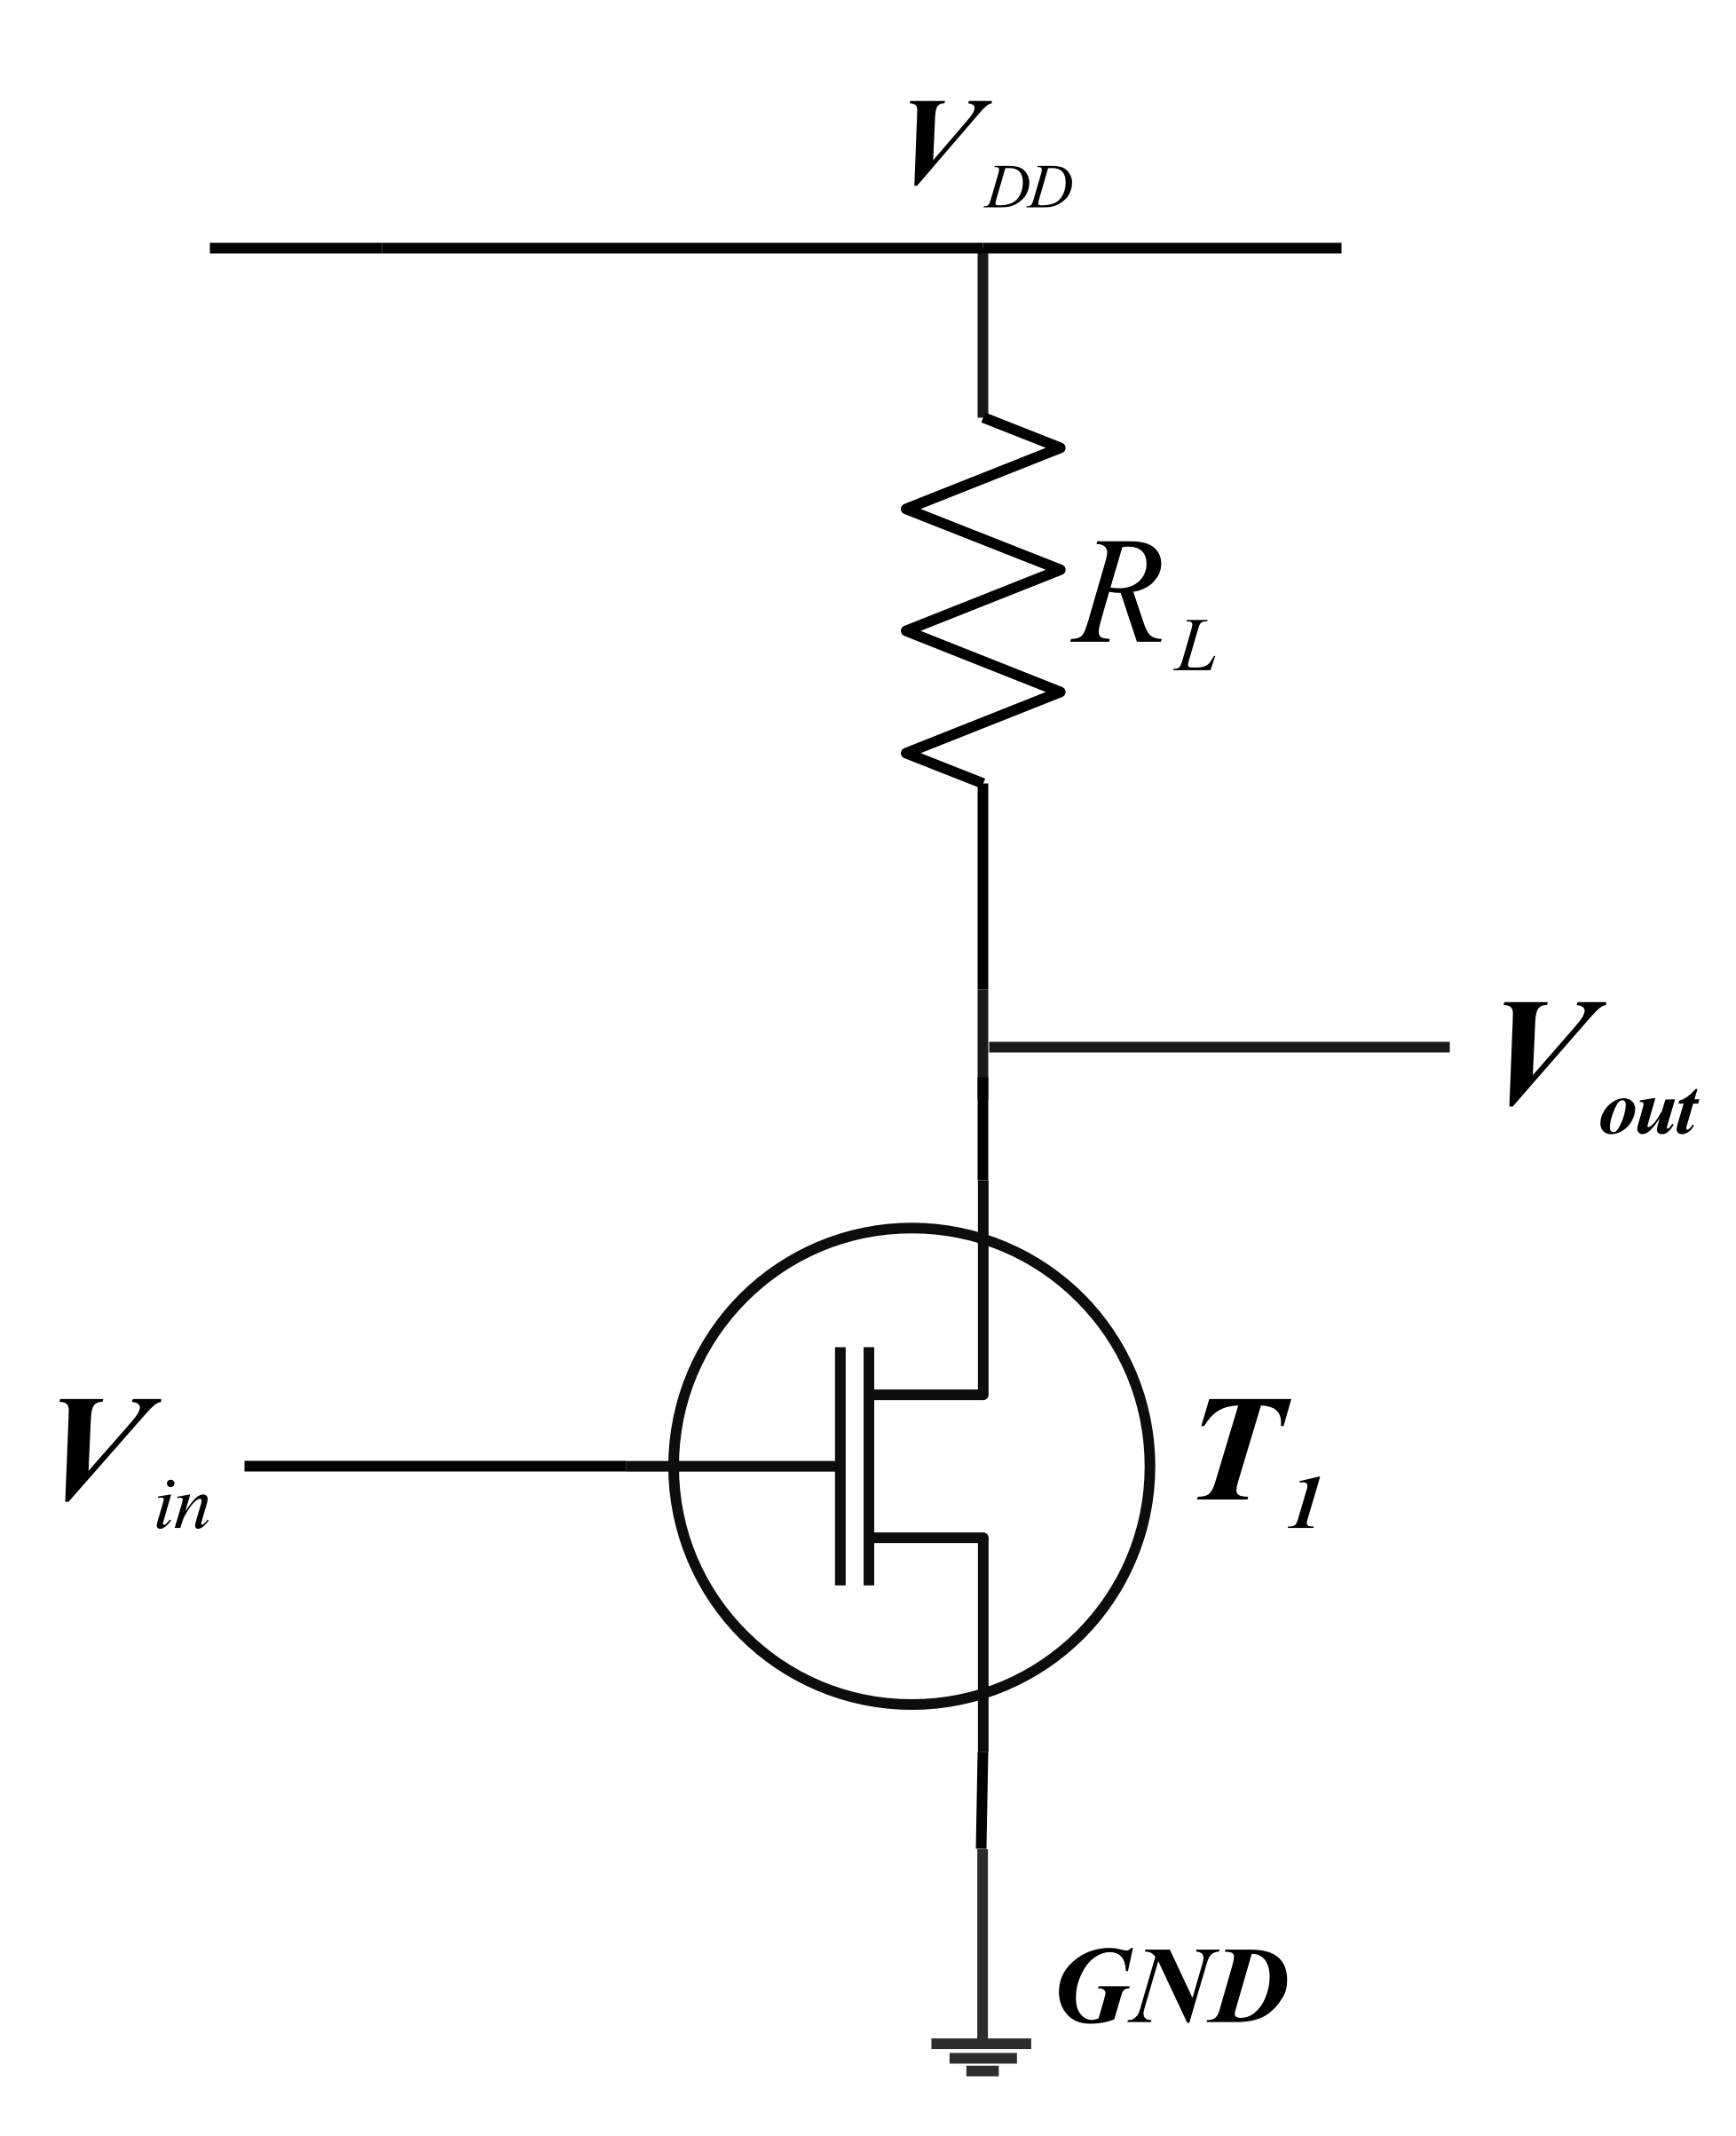
\includegraphics[width=0.45\linewidth]{../EXP04_EEE2214/Images/mos/2}
	\caption{}
	\label{fig:1}
\end{figure}
- When the input \(V_{in}\) is low (logic '0'), \(M_1\) is OFF, and the output \(V_{out}\) is pulled high to \(V_{DD}\).\\
- When \(V_{in}\) is high (logic '1'), \(M_1\) turns ON, pulling \(V_{out}\) low to 0V.

The output voltage \( V_{out} \) is given by:

\[
V_{out} = V_{DD} - I_{D} \cdot R
\]

where:
- \( I_{D} \) is the drain current through the nMOS transistor.

The resistive load leads to higher power dissipation, as there is a direct current path from \( V_{DD} \) to ground when \( M_1 \) is ON. Additionally, the switching speed is limited by the time constant:

\[
\tau = R \cdot C_{out}
\]

where:
- \( C_{out} \) is the output capacitance.
\newpage
	\subsection{Implemention of Gate Using nMOS Inverters}
	\subsubsection{nMOS Inverter using Enhancement Load}
	
	\begin{figure}[H]
		\centering
		
		\begin{subfigure}[t]{0.49\textwidth}
			\centering
			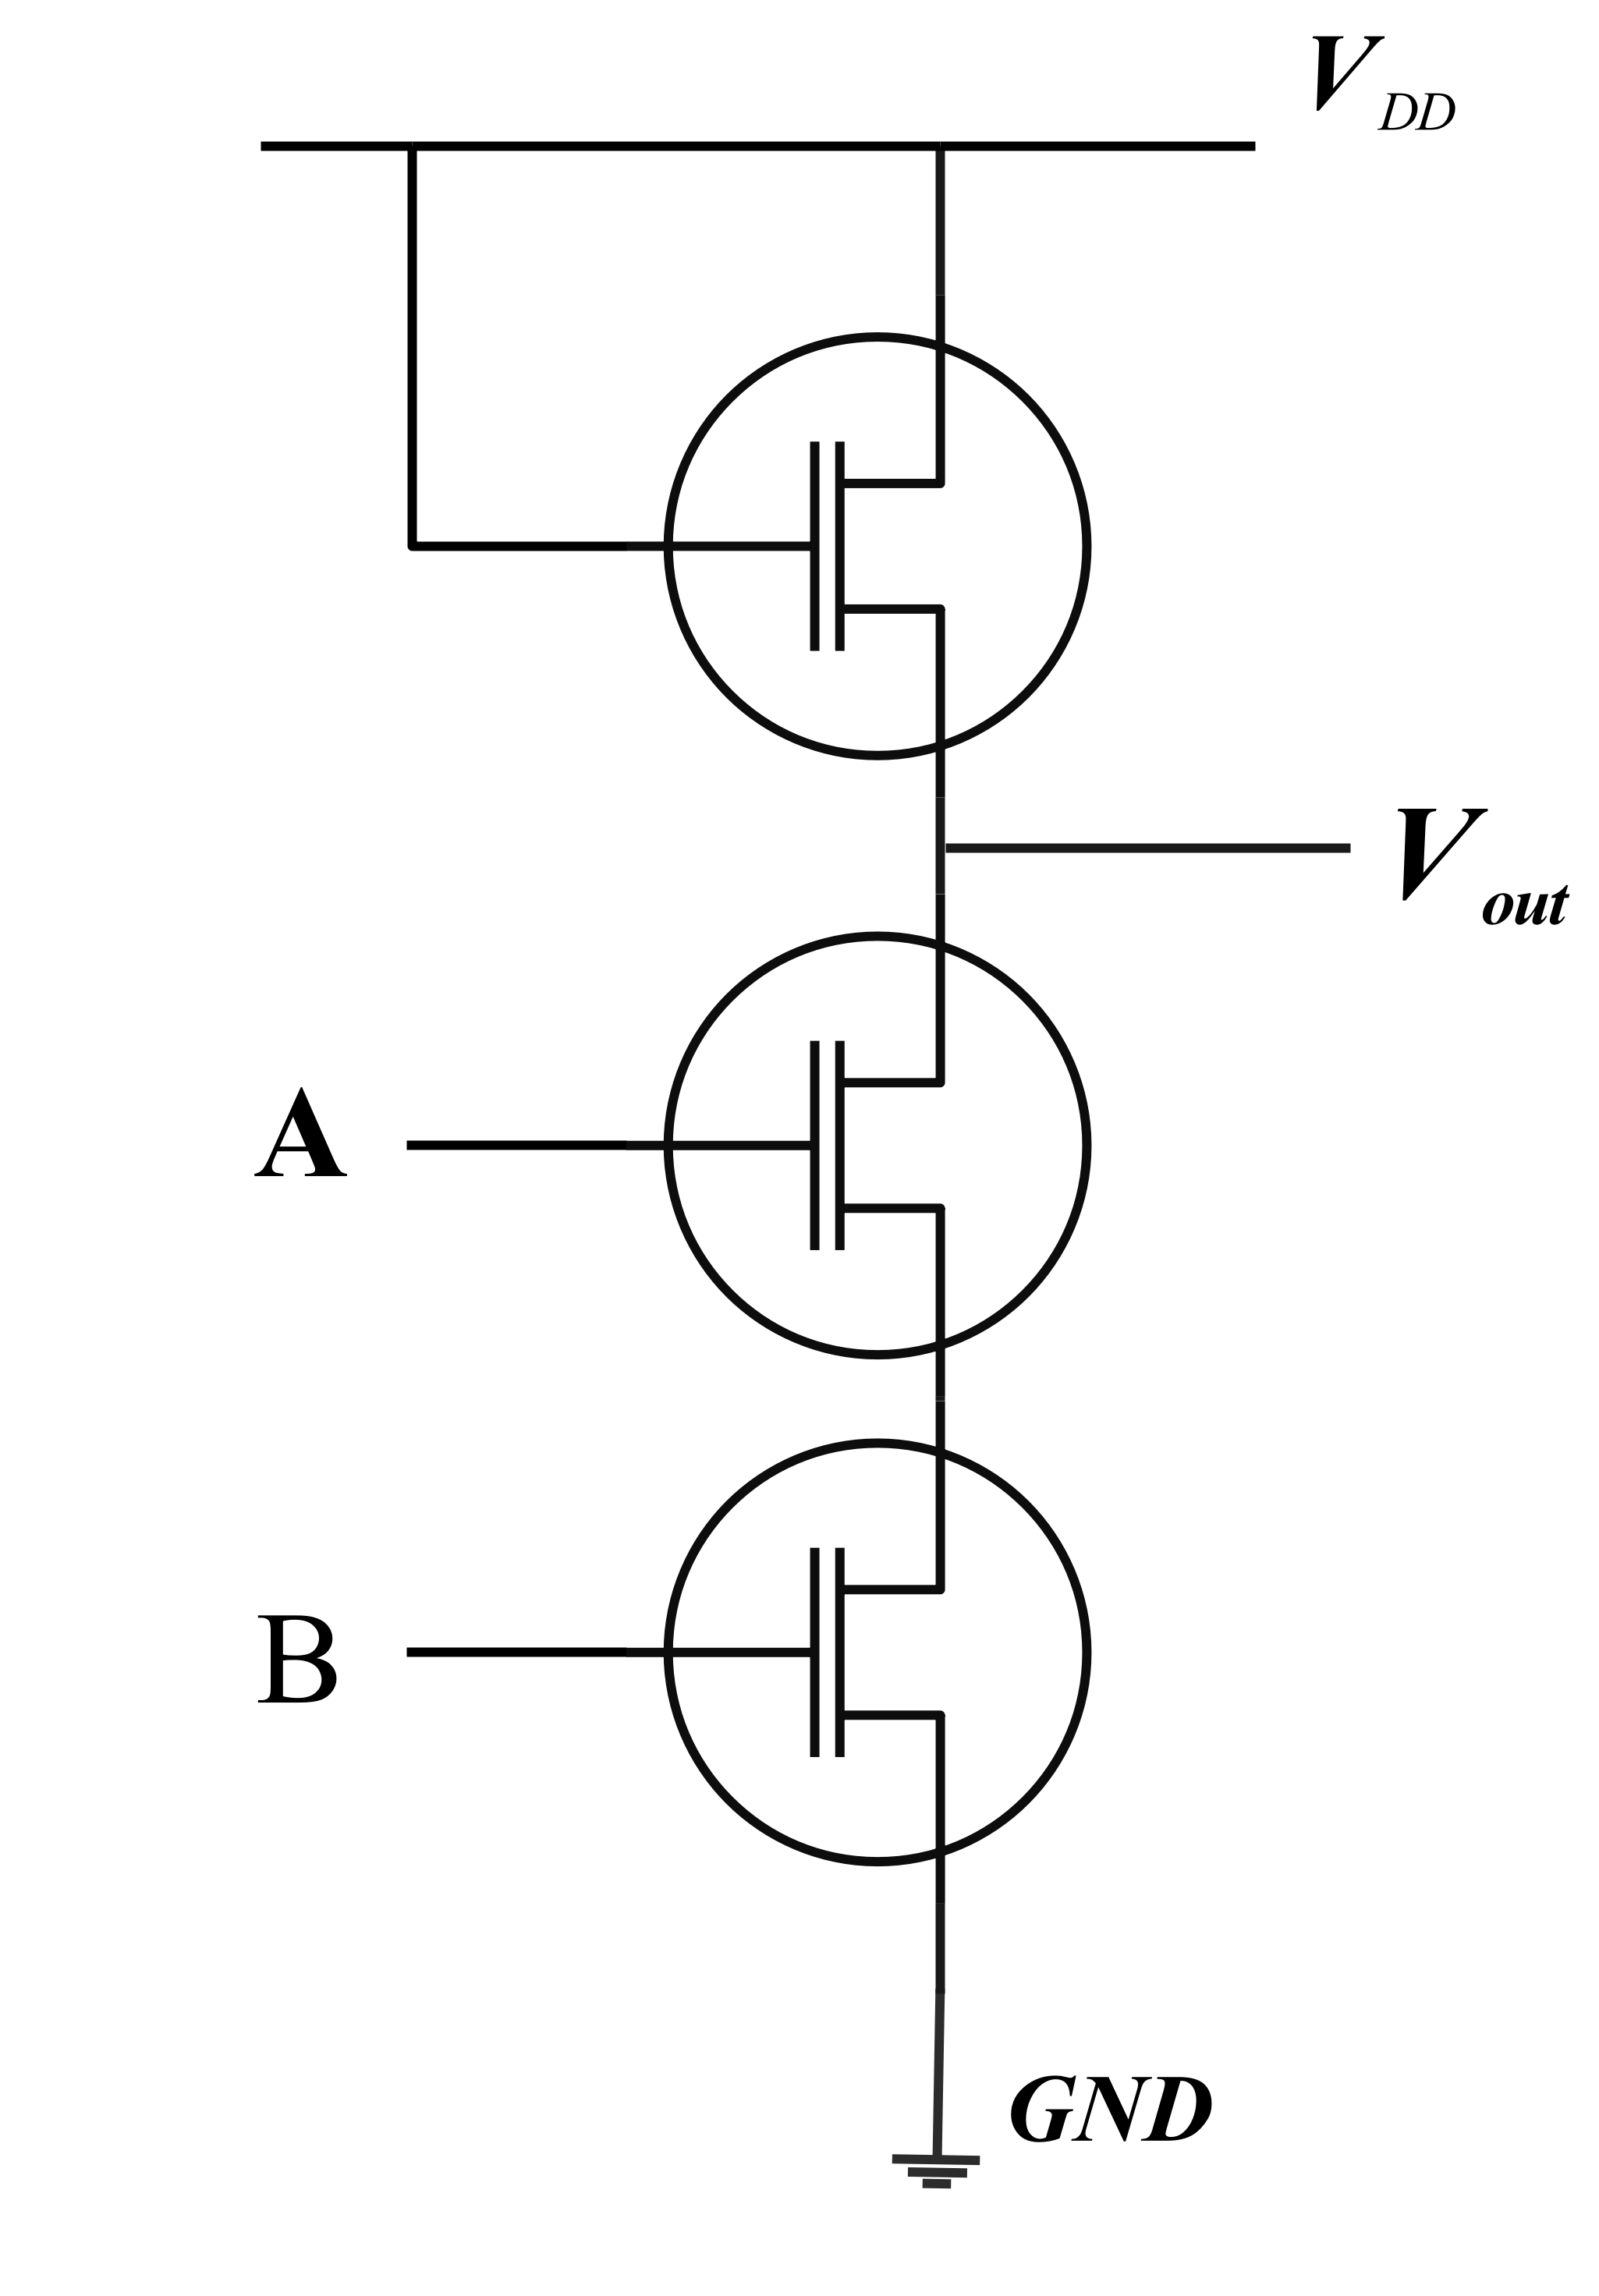
\includegraphics[width=0.7\linewidth]{../EXP04_EEE2214/Images/mos/3}
			
			\caption{NAND-Gate}
			
			\label{fig:ci1}
		\end{subfigure}
		\hfill
		\begin{subfigure}[t]{0.49\textwidth}
			\centering
			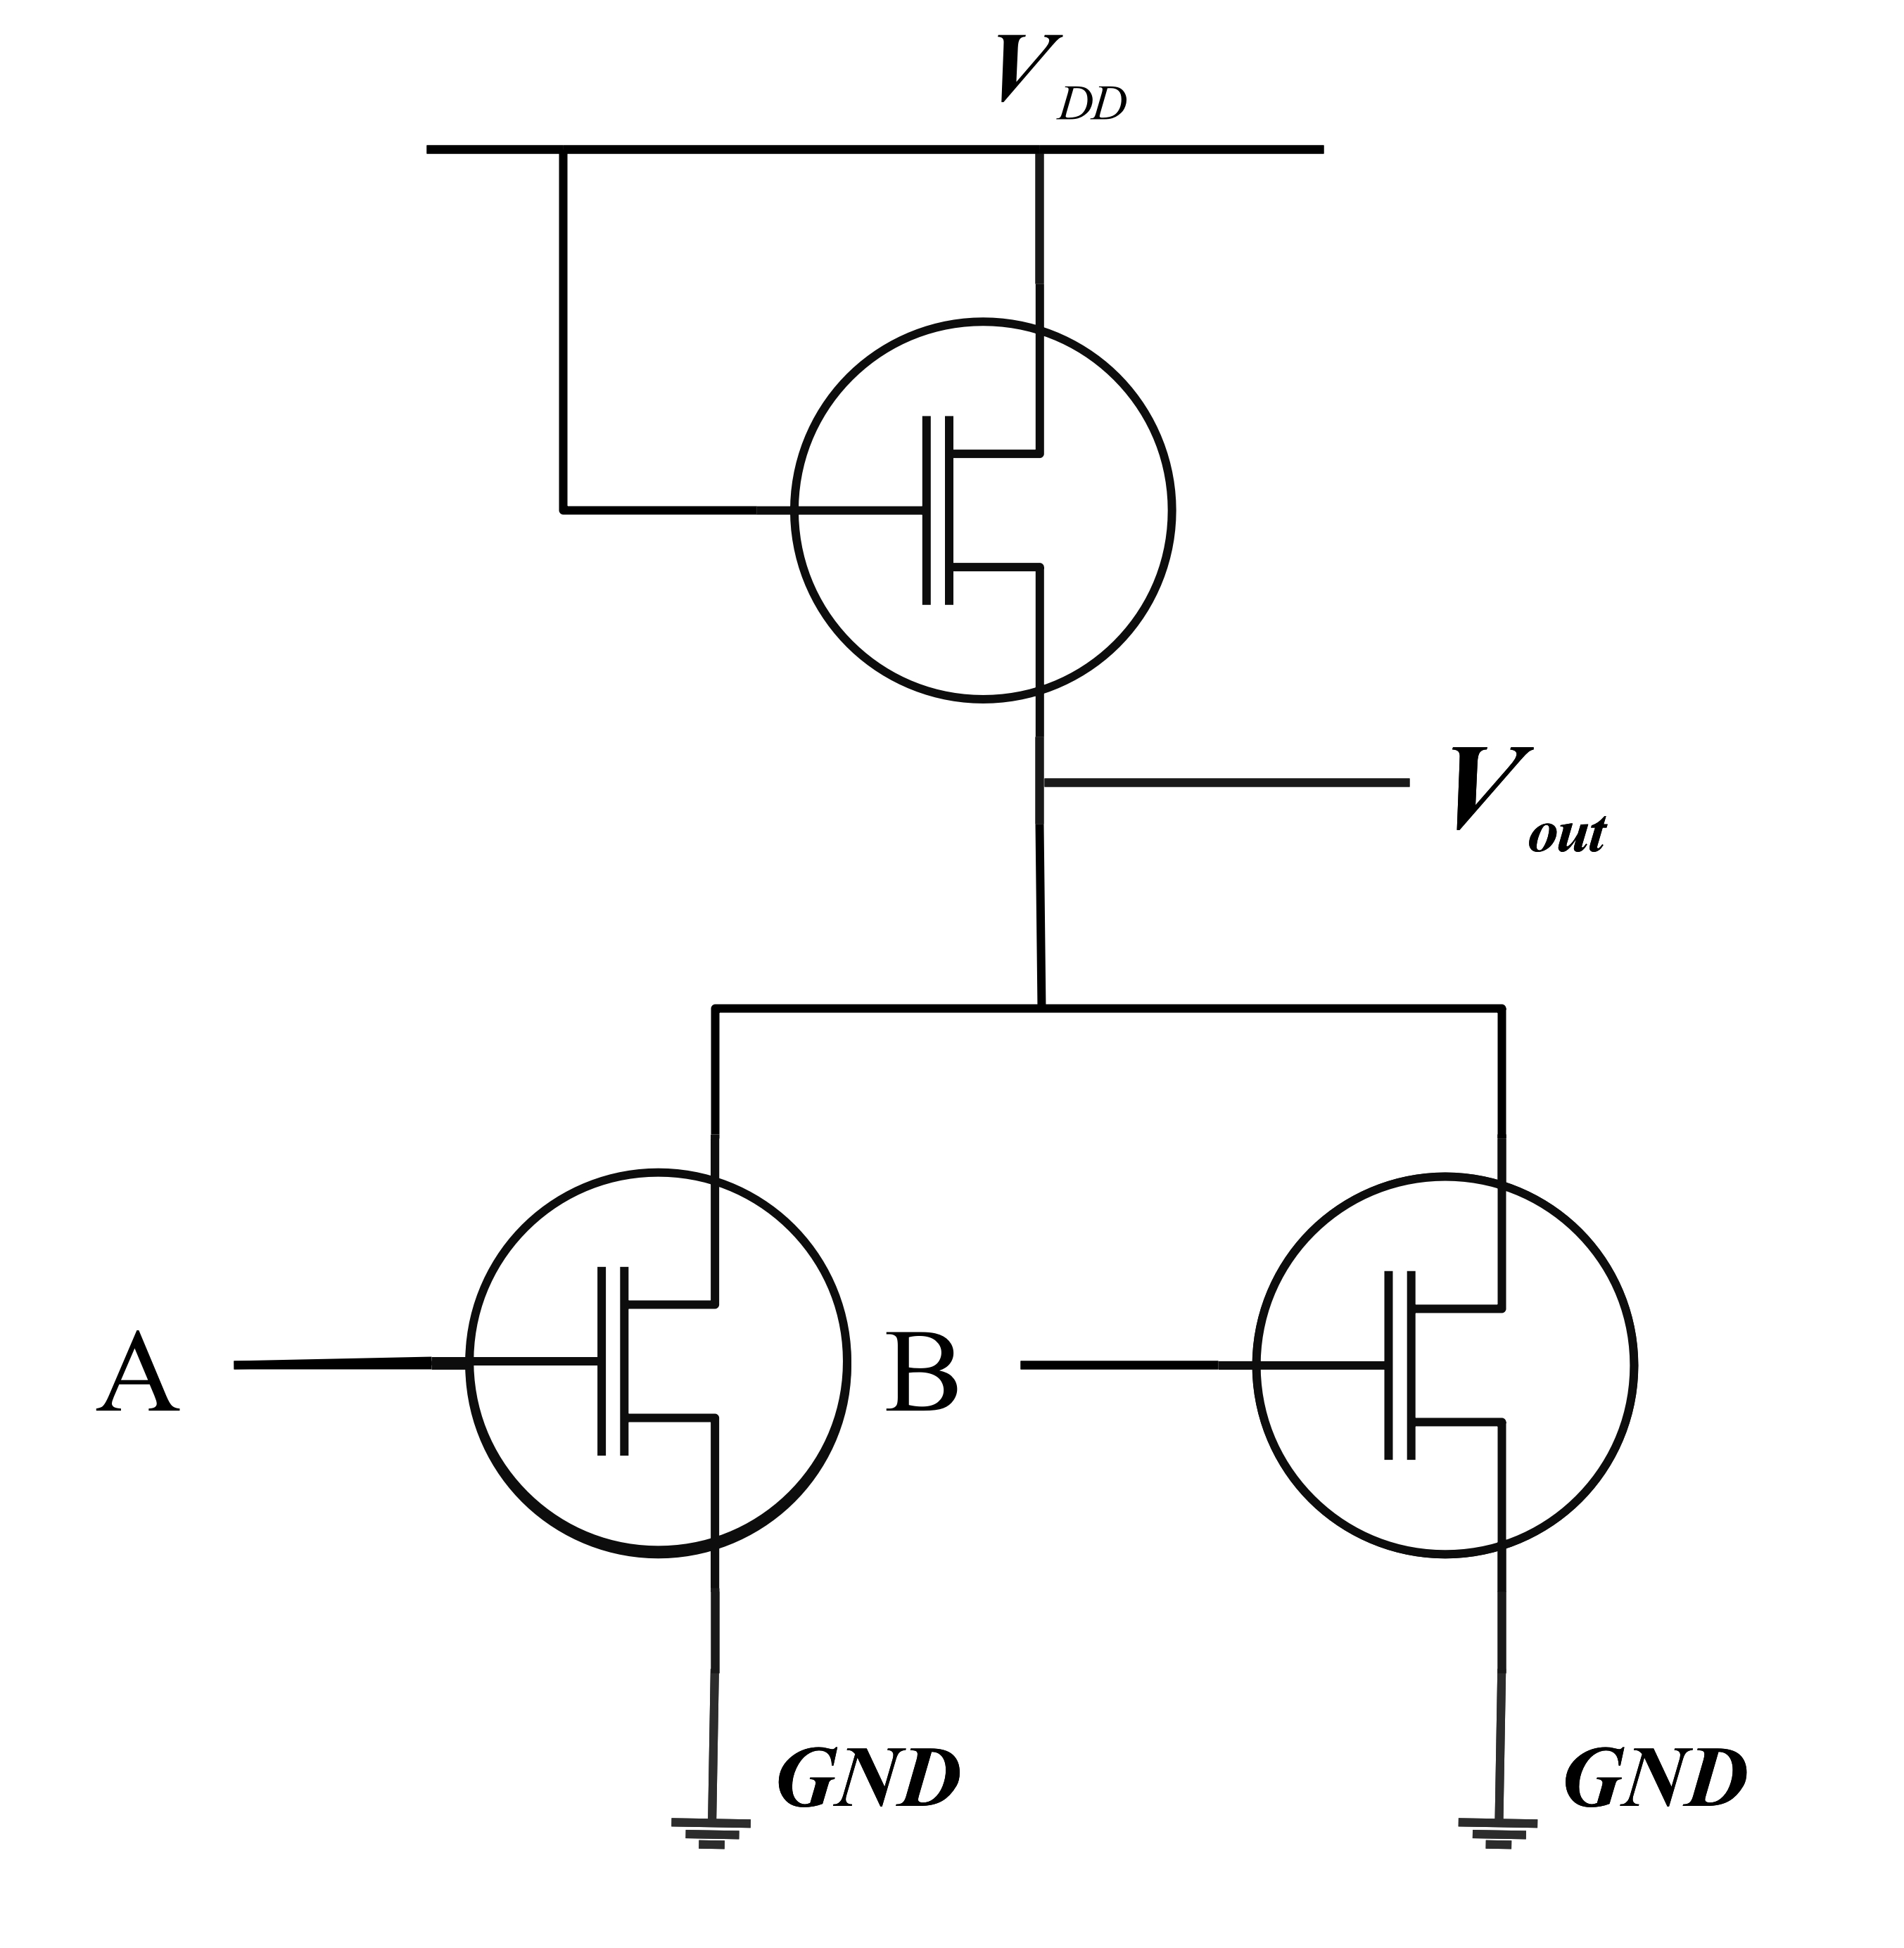
\includegraphics[width=1\linewidth]{../EXP04_EEE2214/Images/mos/4}
			\caption{NOR-Gate}
			\label{fig:ci1}
		\end{subfigure}
		\caption{Circuit Diagram of NAND-Gate \& NOR-Gate using nMOS Inverter with Enhancement Load}
	\end{figure}
	
	
	
		\subsubsection{nMOS Inverter using Resistive Load}
		
		\begin{figure}[H]
			\centering
			
			\begin{subfigure}[t]{0.49\textwidth}
				\centering
				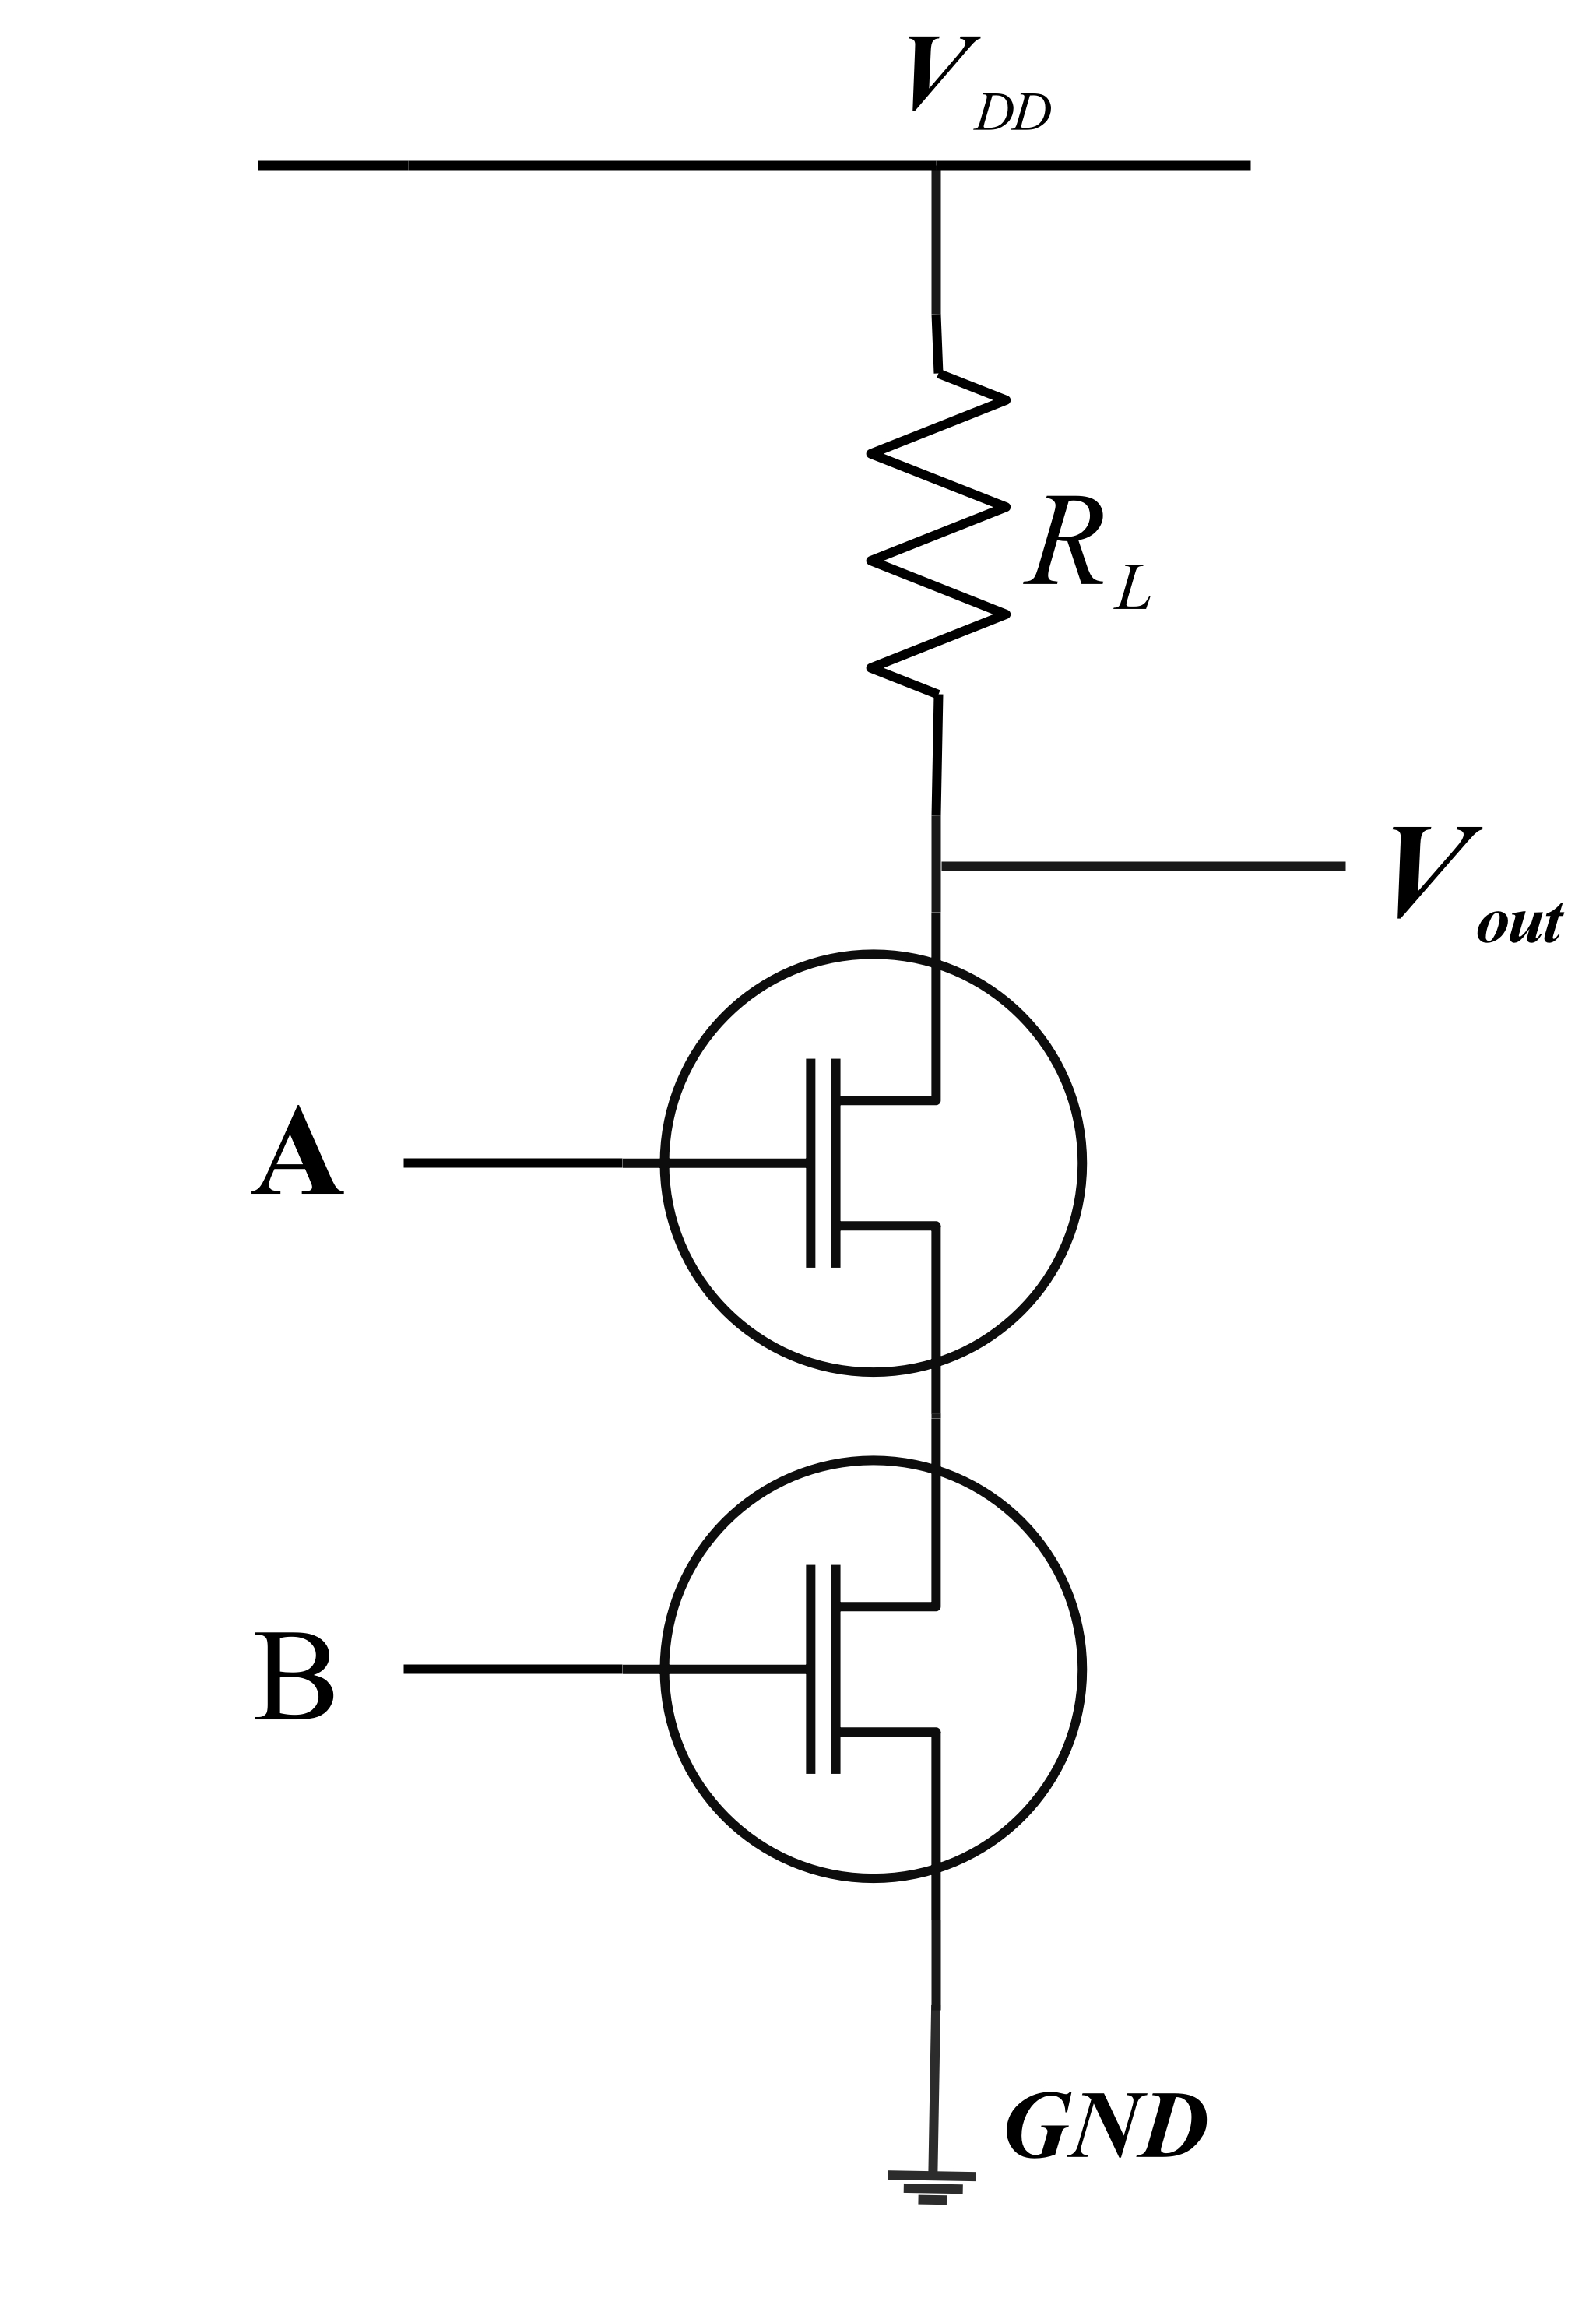
\includegraphics[width=.7\linewidth]{../EXP04_EEE2214/Images/mos/6}
				
				\caption{NAND-Gate}
				
				\label{fig:ci1}
			\end{subfigure}
			\hfill
			\begin{subfigure}[t]{0.49\textwidth}
				\centering
				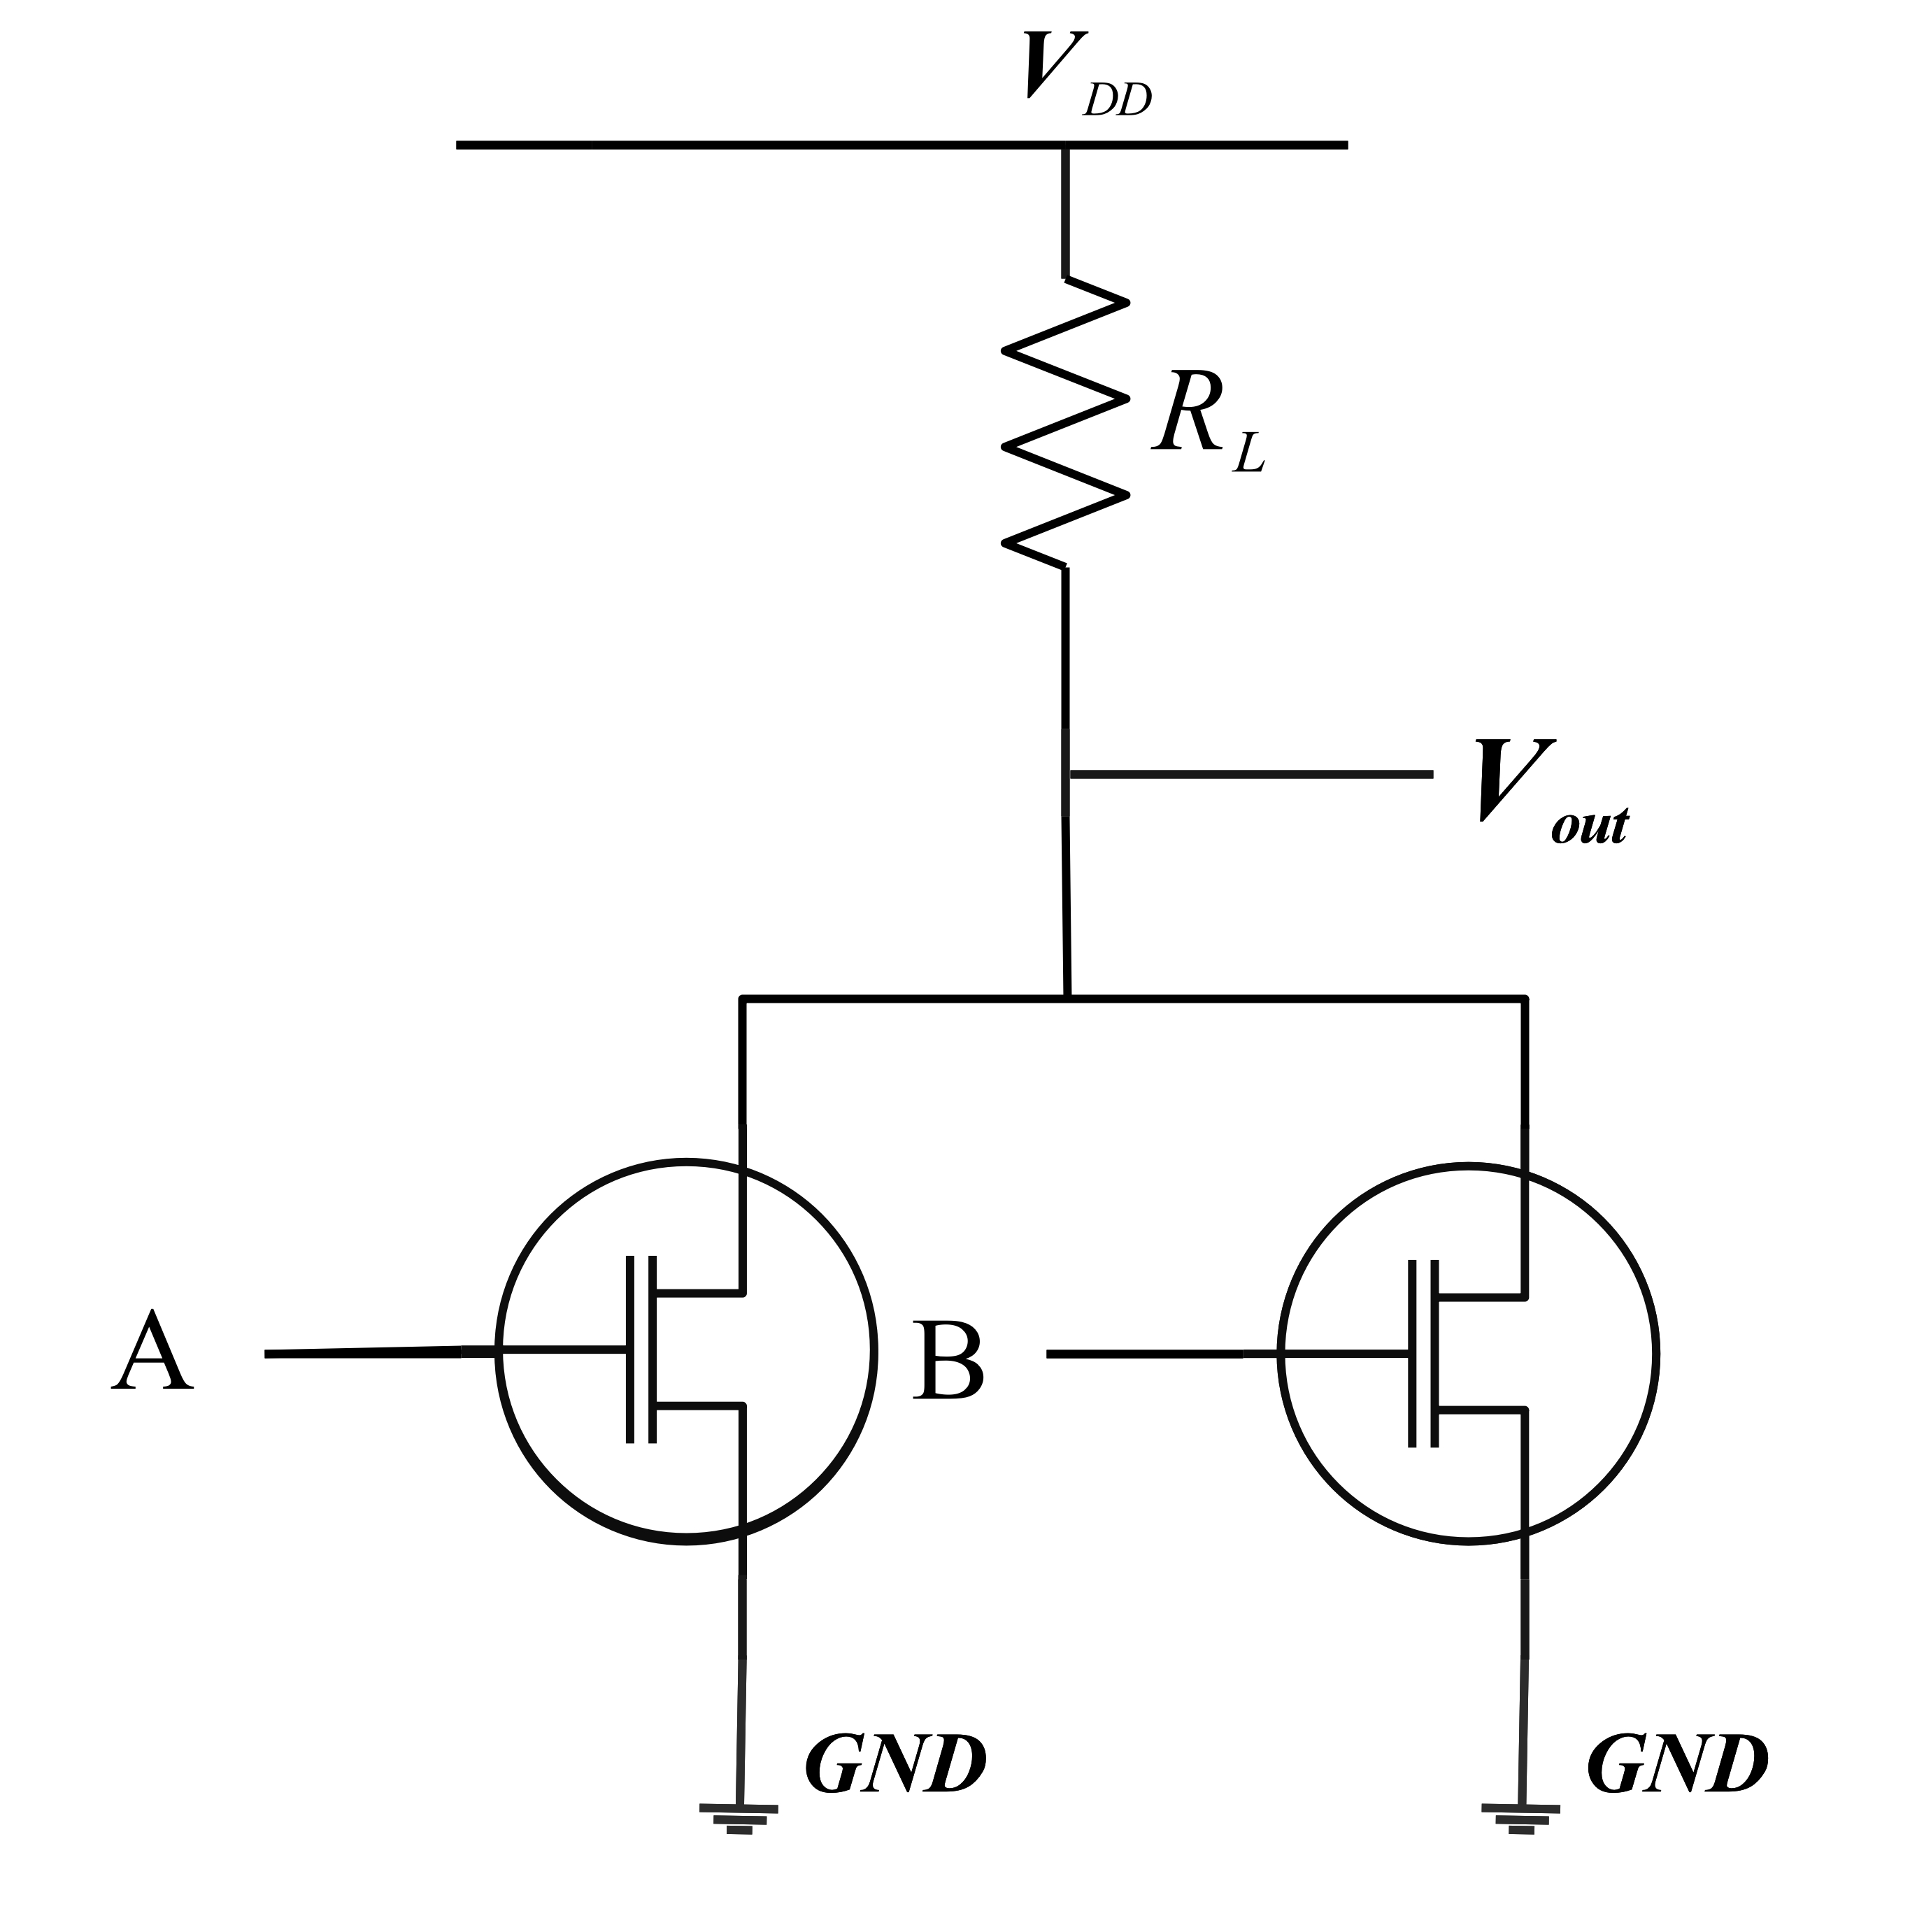
\includegraphics[width=1\linewidth]{../EXP04_EEE2214/Images/mos/5}
				\caption{NOR-Gate}
				\label{fig:ci1}
			\end{subfigure}
			\caption{Circuit Diagram of NAND-Gate \& NOR-Gate using nMOS Inverter with Resistive Load}
		\end{figure}
	\newpage
	\section{Schematic Layout }
\subsection{NAND-Gate using nMOS Inverter with Enhancement Load}
\begin{figure}[H]
	\centering
	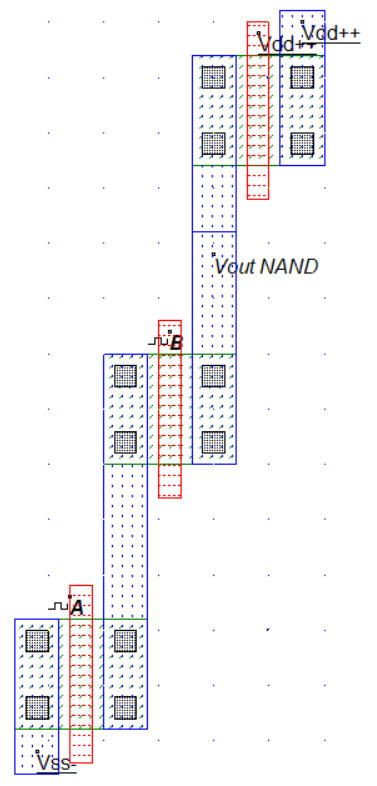
\includegraphics[width=0.6\linewidth]{Images5/1}
	\caption{Design layout of NAND-Gate using nMOS Inverter with Enhancement Load}
	\label{fig:1}
\end{figure}
\subsection{NOR-Gate using nMOS Inverter with Enhancement Load}
	\begin{figure}[H]
		\centering
		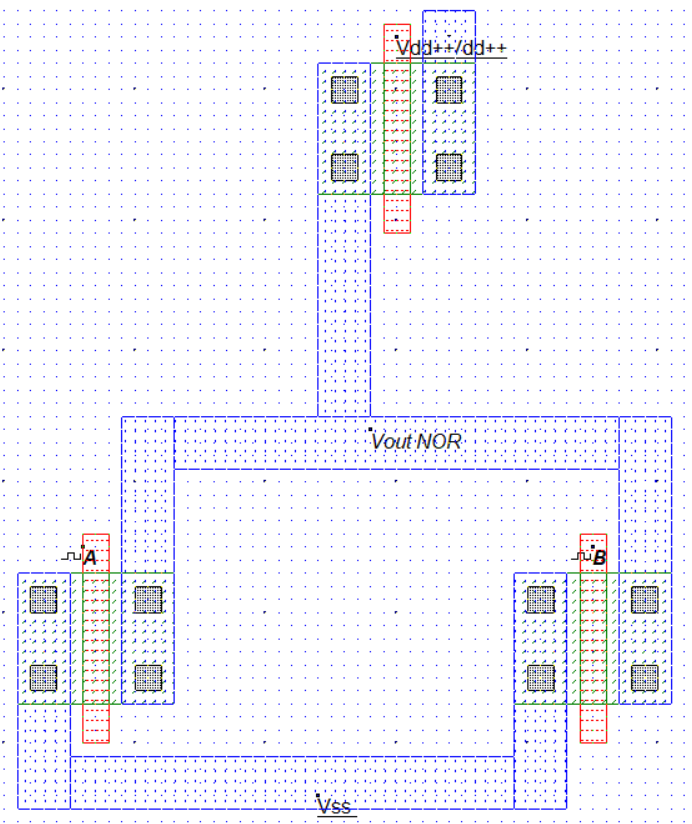
\includegraphics[width=1\linewidth]{Images5/2}
		\caption{Design layout of NOR-Gate using nMOS Inverter with Enhancement Load}
		\label{fig:1}
	\end{figure}
	
	\subsection{NAND-Gate \& NOR-Gate using nMOS Inverter with Resistive Load}
\begin{figure}[H]
	\centering
	
	\begin{subfigure}[t]{0.49\textwidth}
		\centering
		
		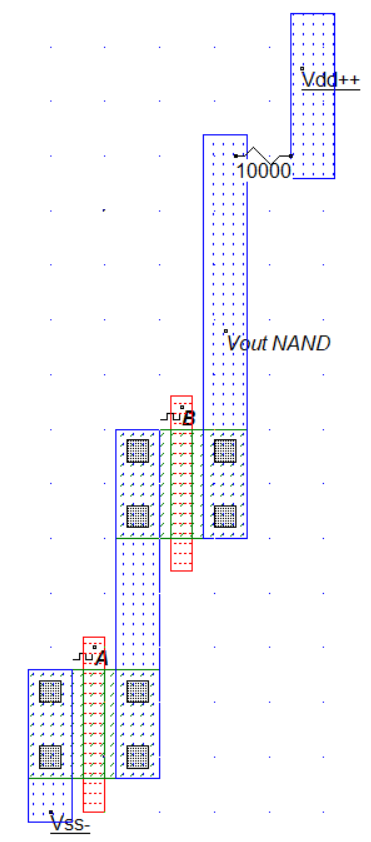
\includegraphics[width=.91\linewidth]{Images5/3}
		
		\caption{NAND-Gate}
		
		\label{fig:ci1}
	\end{subfigure}
	\hfill
	\begin{subfigure}[t]{0.49\textwidth}
		\centering
		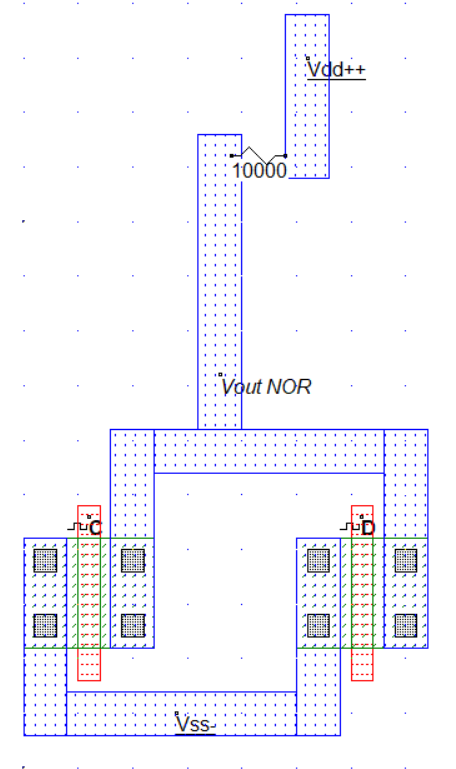
\includegraphics[width=1.2\linewidth]{Images5/4}
		\caption{NOR-Gate}
		\label{fig:ci1}
	\end{subfigure}
	\caption{Design layout of NAND-Gate \& NOR-Gate using nMOS Inverter with Resistive Load}
\end{figure}

	
	
	\section{Specification}
	\begin{table}[H]
		\centering
		\caption{MOSFET Dimensions for nMOS and pMOS Transistors}
		\label{tab:MOSFET_dimensions}
		\begin{tabular}{|c|c|c|c|c|}
			\hline
			\textbf{MOS} & \textbf{\begin{tabular}[c]{@{}c@{}}Width\\ ($\mu m$)\end{tabular}} & \textbf{\begin{tabular}[c]{@{}c@{}}Length\\ ($\mu m$)\end{tabular}} & \textbf{\begin{tabular}[c]{@{}c@{}}Width\\ ($\lambda$)\end{tabular}} & \textbf{\begin{tabular}[c]{@{}c@{}}Length\\ ($\lambda$)\end{tabular}} \\ \hline
			nMOS & 0.600 & 0.120 & 10 & 2 \\ \hline
			pMOS & 0.600 & 0.120 & 10 & 2 \\ \hline
		\end{tabular}
		
	\end{table}
	
	\begin{table}[H]
		\centering
		\caption{Parameters of Input Clock Signal for 1 Finger NAND-Gate and AND-Gate}
		% Sub-table (a)
		\begin{subtable}[t]{0.48\textwidth} % Adjusted width for each sub-table
			\centering
			\begin{tabular}{|c|c|c|}
				\hline
				\textbf{Parameter}          & \textbf{Value} & \textbf{Unit} \\ \hline
				High Level $(V)$            & 5.00           & $V$           \\ \hline
				Low Level $(V)$             & 0.00           & $V$           \\ \hline
				Time Low $(tl)$             & 0.225          & $ns$          \\ \hline
				Rise Time $(tr)$            & 0.002          & $ns$          \\ \hline
				Time High $(th)$            & 0.225          & $ns$          \\ \hline
				Fall Time $(tf)$            & 0.002          & $ns$          \\ \hline
			\end{tabular}
			\caption{Input clock signal of A} % Sub-table (a) caption
		\end{subtable}
		\hfil
		% Sub-table (b)
		\begin{subtable}[t]{0.48\textwidth} % Adjusted width for each sub-table
			\centering
			\begin{tabular}{|c|c|c|}
				\hline
				\textbf{Parameter}          & \textbf{Value} & \textbf{Unit} \\ \hline
				High Level $(V)$            & 5.00           & $V$           \\ \hline
				Low Level $(V)$             & 0.00           & $V$           \\ \hline
				Time Low $(tl)$             & 0.452         & $ns$          \\ \hline
				Rise Time $(tr)$            & 0.002          & $ns$          \\ \hline
				Time High $(th)$            & 0.452          & $ns$          \\ \hline
				Fall Time $(tf)$            & 0.002          & $ns$          \\ \hline
			\end{tabular}
			\caption{Input clock signal of B} % Sub-table (b) caption
		\end{subtable}
	\end{table}
	
	\begin{table}[H]
		\centering
		\caption{Parameters of Input Clock Signal for 2 Finger NAND-Gate and AND-Gate}
		% Sub-table (a)
		\begin{subtable}[t]{0.48\textwidth} % Adjusted width for each sub-table
			\centering
			\begin{tabular}{|c|c|c|}
				\hline
				\textbf{Parameter}          & \textbf{Value} & \textbf{Unit} \\ \hline
				High Level $(V)$            & 5.00           & $V$           \\ \hline
				Low Level $(V)$             & 0.00           & $V$           \\ \hline
				Time Low $(tl)$             & 0.452         & $ns$          \\ \hline
				Rise Time $(tr)$            & 0.002          & $ns$          \\ \hline
				Time High $(th)$            & 0.452          & $ns$          \\ \hline
				Fall Time $(tf)$            & 0.002          & $ns$          \\ \hline
			\end{tabular}
			\caption{Input clock signal of A} % Sub-table (a) caption
		\end{subtable}
		\hfil
		% Sub-table (b)
		\begin{subtable}[t]{0.48\textwidth} % Adjusted width for each sub-table
			\centering
			\begin{tabular}{|c|c|c|}
				\hline
				\textbf{Parameter}          & \textbf{Value} & \textbf{Unit} \\ \hline
				High Level $(V)$            & 5.00           & $V$           \\ \hline
				Low Level $(V)$             & 0.00           & $V$           \\ \hline
				Time Low $(tl)$             & 0.225          & $ns$          \\ \hline
				Rise Time $(tr)$            & 0.002          & $ns$          \\ \hline
				Time High $(th)$            & 0.225          & $ns$          \\ \hline
				Fall Time $(tf)$            & 0.002          & $ns$          \\ \hline
			\end{tabular}
			\caption{Input clock signal of B} % Sub-table (b) caption
		\end{subtable}
		
		
		
	\end{table}
	\begin{table}[H]
		\centering
		\caption{Parameters for Vdd+, Vss- and Load Resistance }
		\begin{tabular}{|c|c|c|}
			\hline
			\textbf{Parameter} & \textbf{Value} & \textbf{Unit} \\ \hline
			Vdd+               & 5.00           & $V $            \\ \hline
			Vss-               & 0.00           & $V$             \\ \hline
			Resistance         & 10000         & $\Omega$             \\ \hline
		\end{tabular}
		
	\end{table}
	
	
	\newpage
	\section{Output Waveshape }
	
	\subsection{nMOS Inverter with Enhancement Load}
\begin{figure}[H]
	\centering
	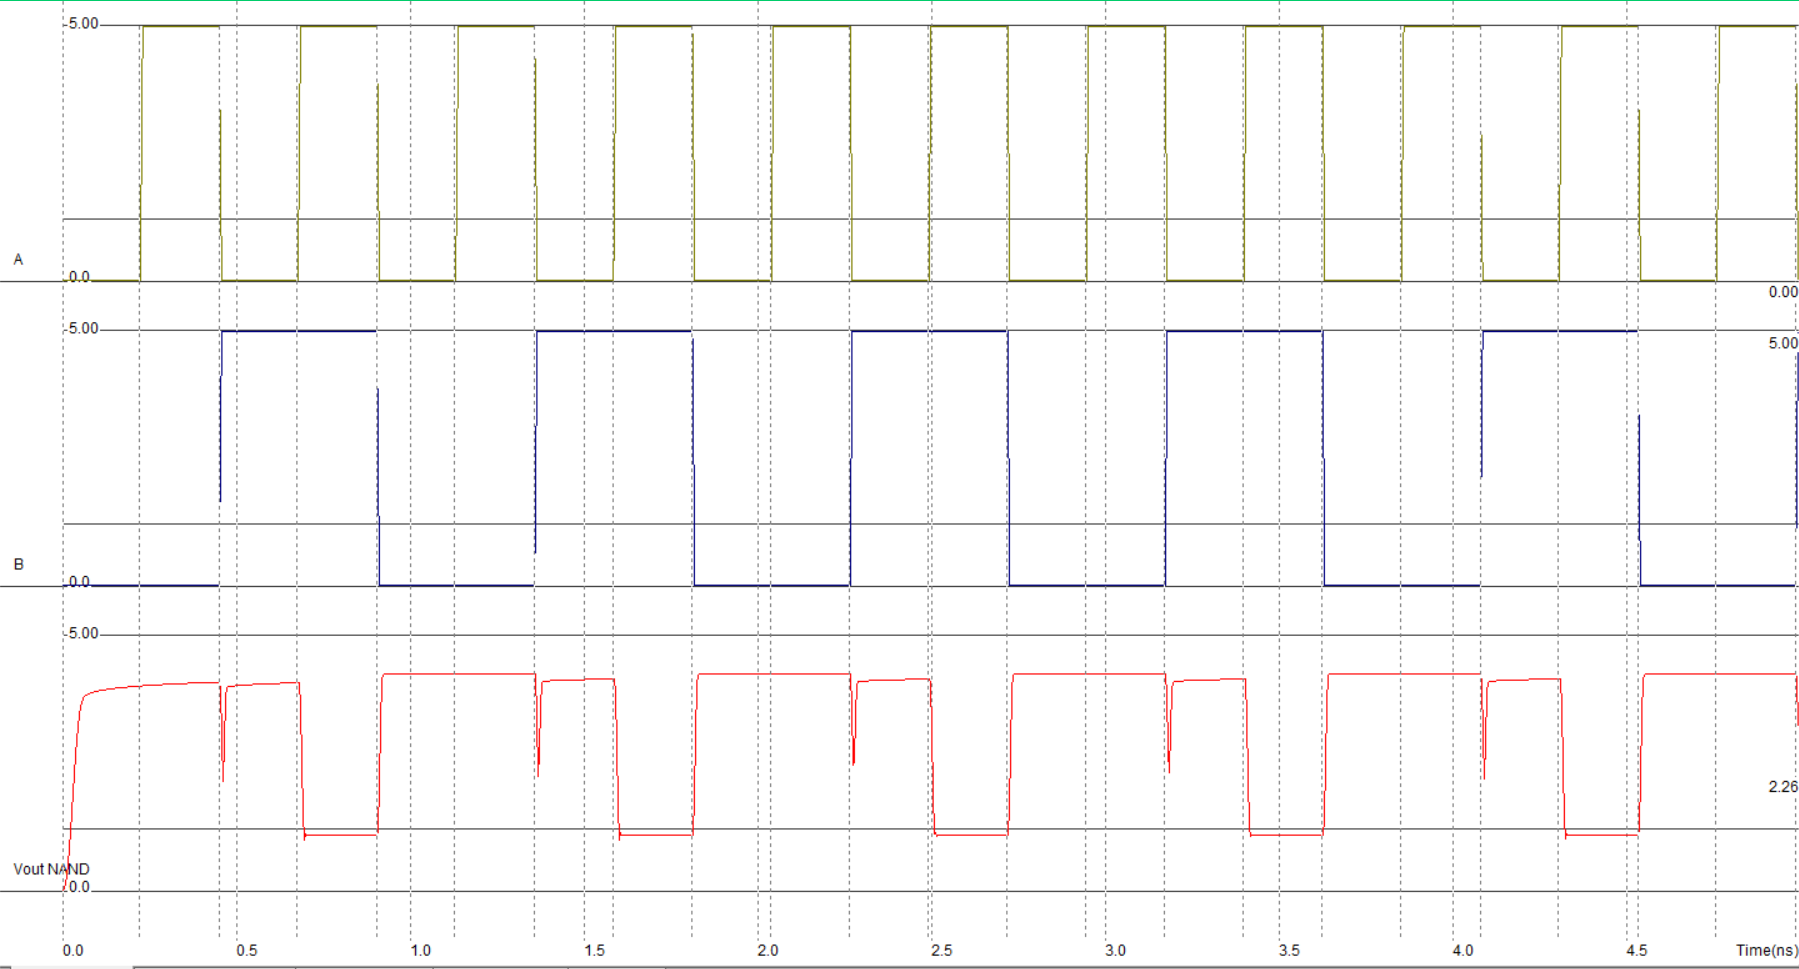
\includegraphics[width=1\linewidth, height=.41\textheight]{Images5/1.1}
	\caption{2 Input NAND-Gate using nMOS Inverter with Enhancement Load}
	\label{fig:1}
\end{figure}

\begin{figure}[H]
	\centering
	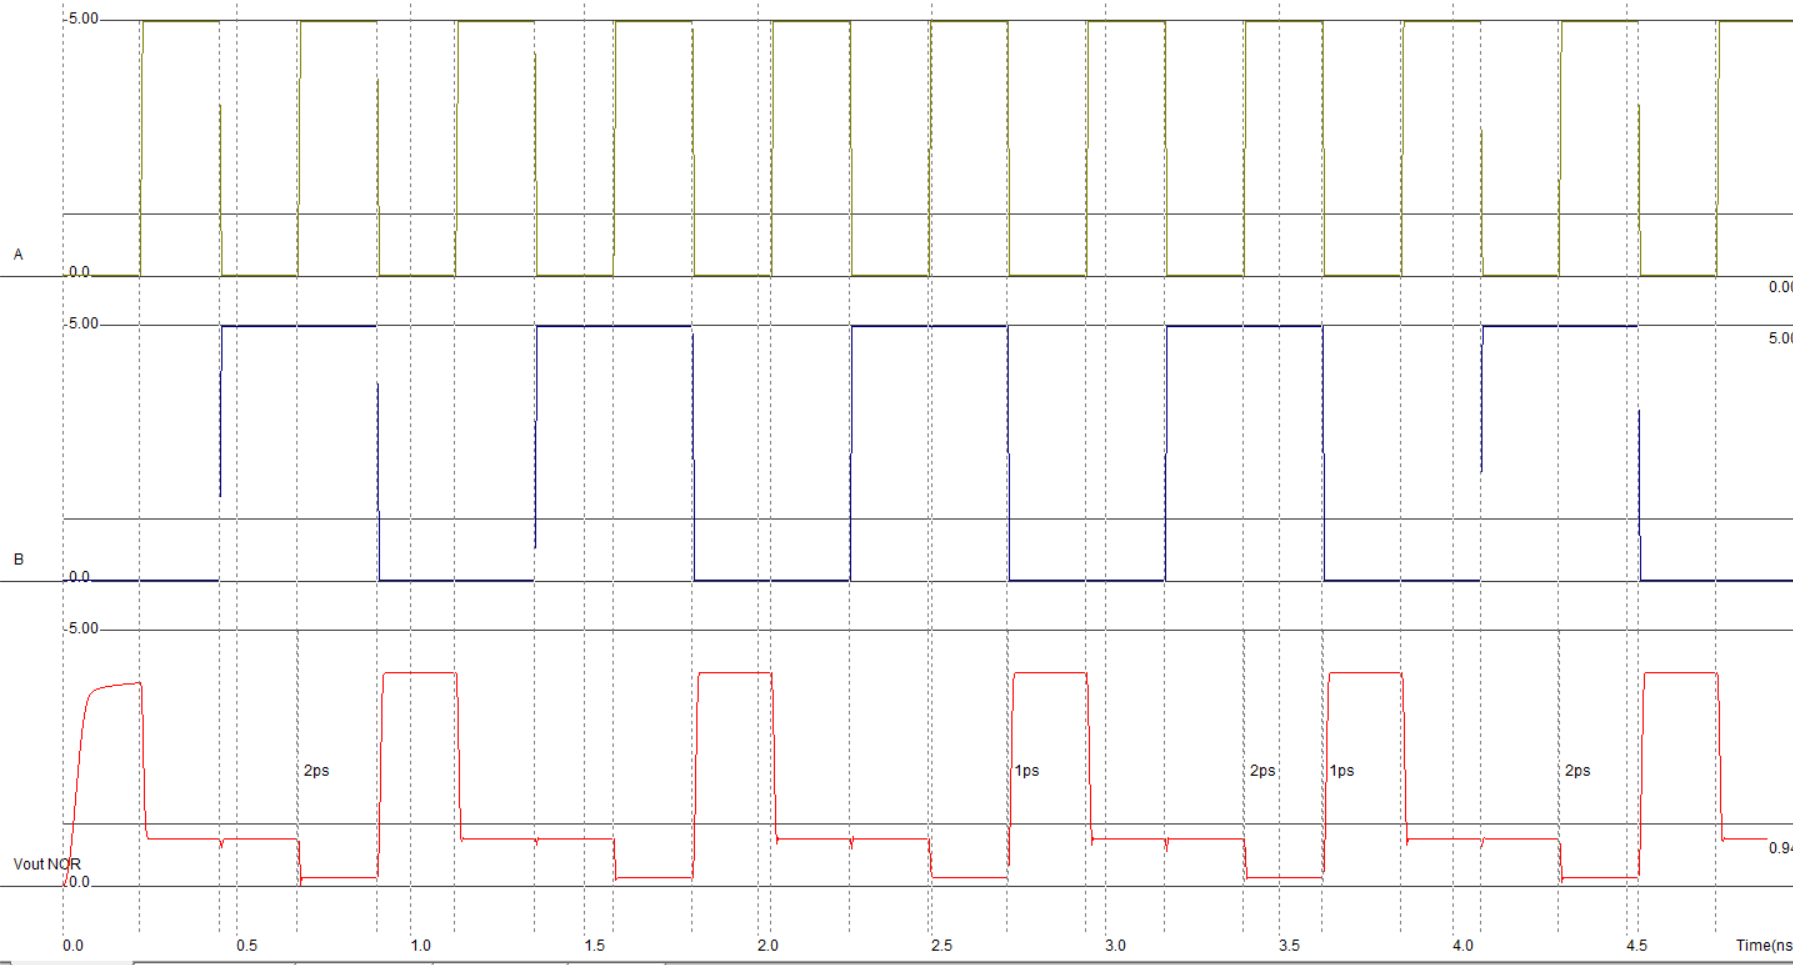
\includegraphics[width=1\linewidth, height=.41\textheight]{Images5/2.1}
	\caption{2 Input NOR-Gate using nMOS Inverter with Enhancement Load}
	\label{fig:1}
\end{figure}
\newpage
\subsection{nMOS Inverter with Resistive Load}
	\begin{figure}[H]
		\centering
		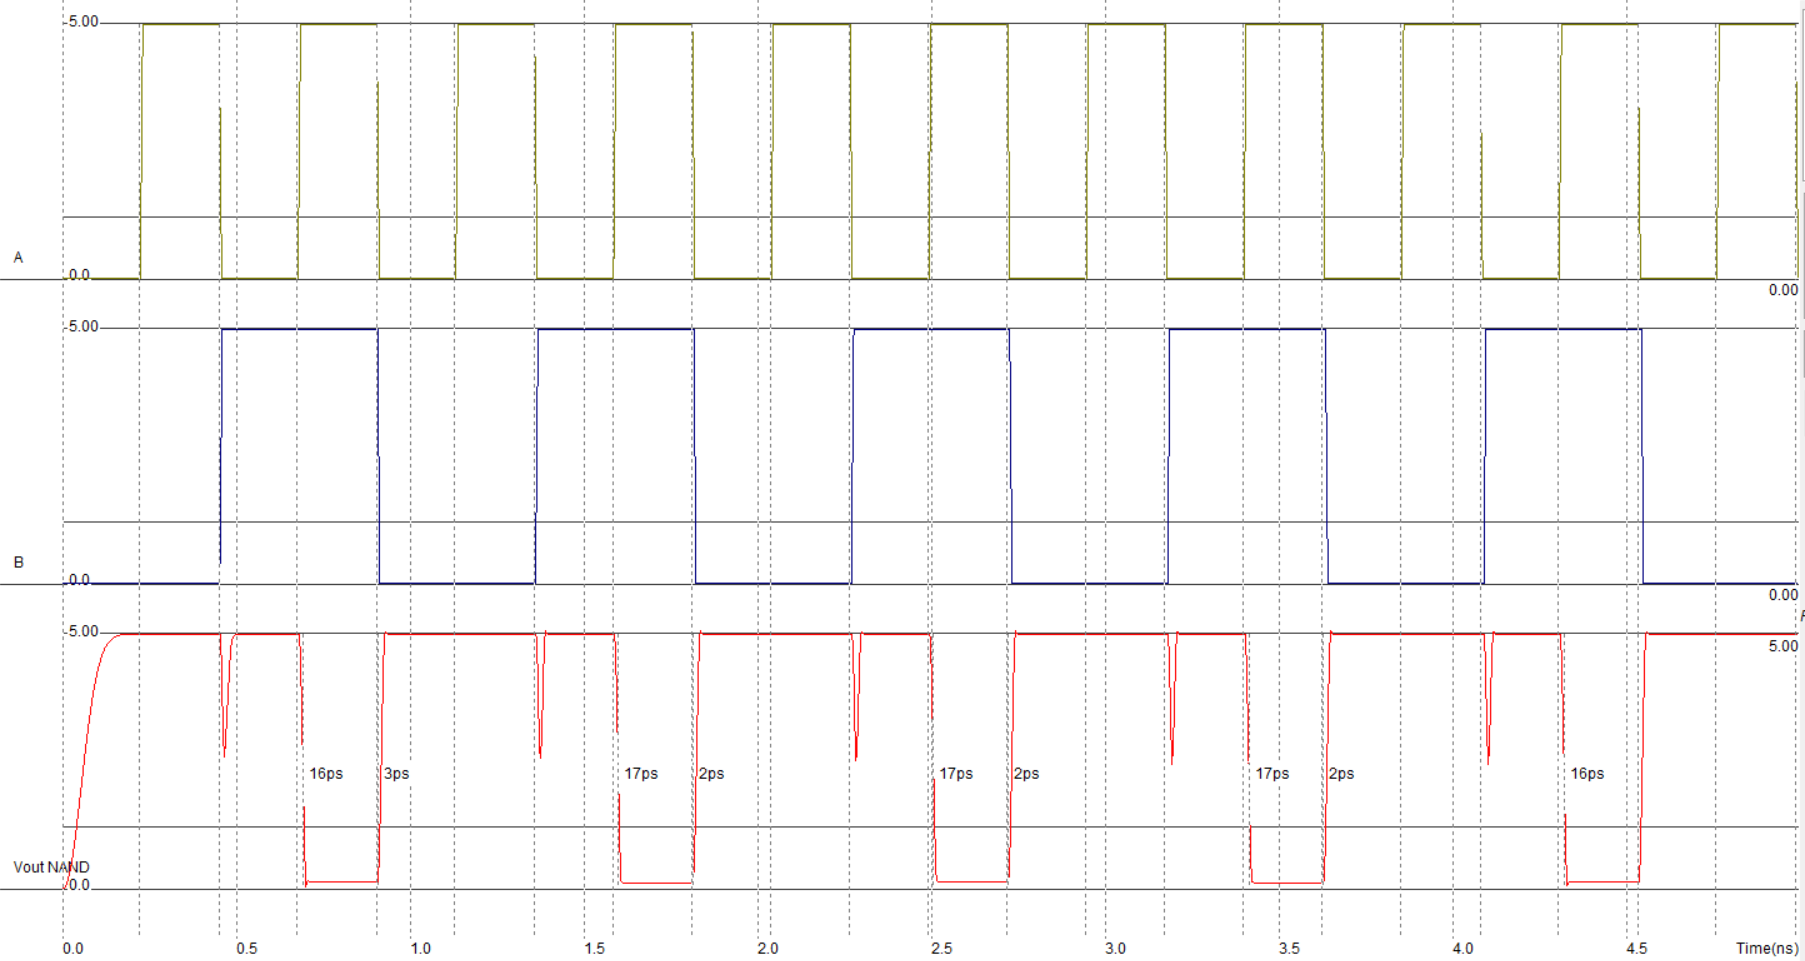
\includegraphics[width=1\linewidth, height=.41\textheight]{Images5/3.1}
		\caption{2 Input NAND-Gate using nMOS Inverter with Resistive Load}
		\label{fig:1}
	\end{figure}
	\begin{figure}[H]
		\centering
		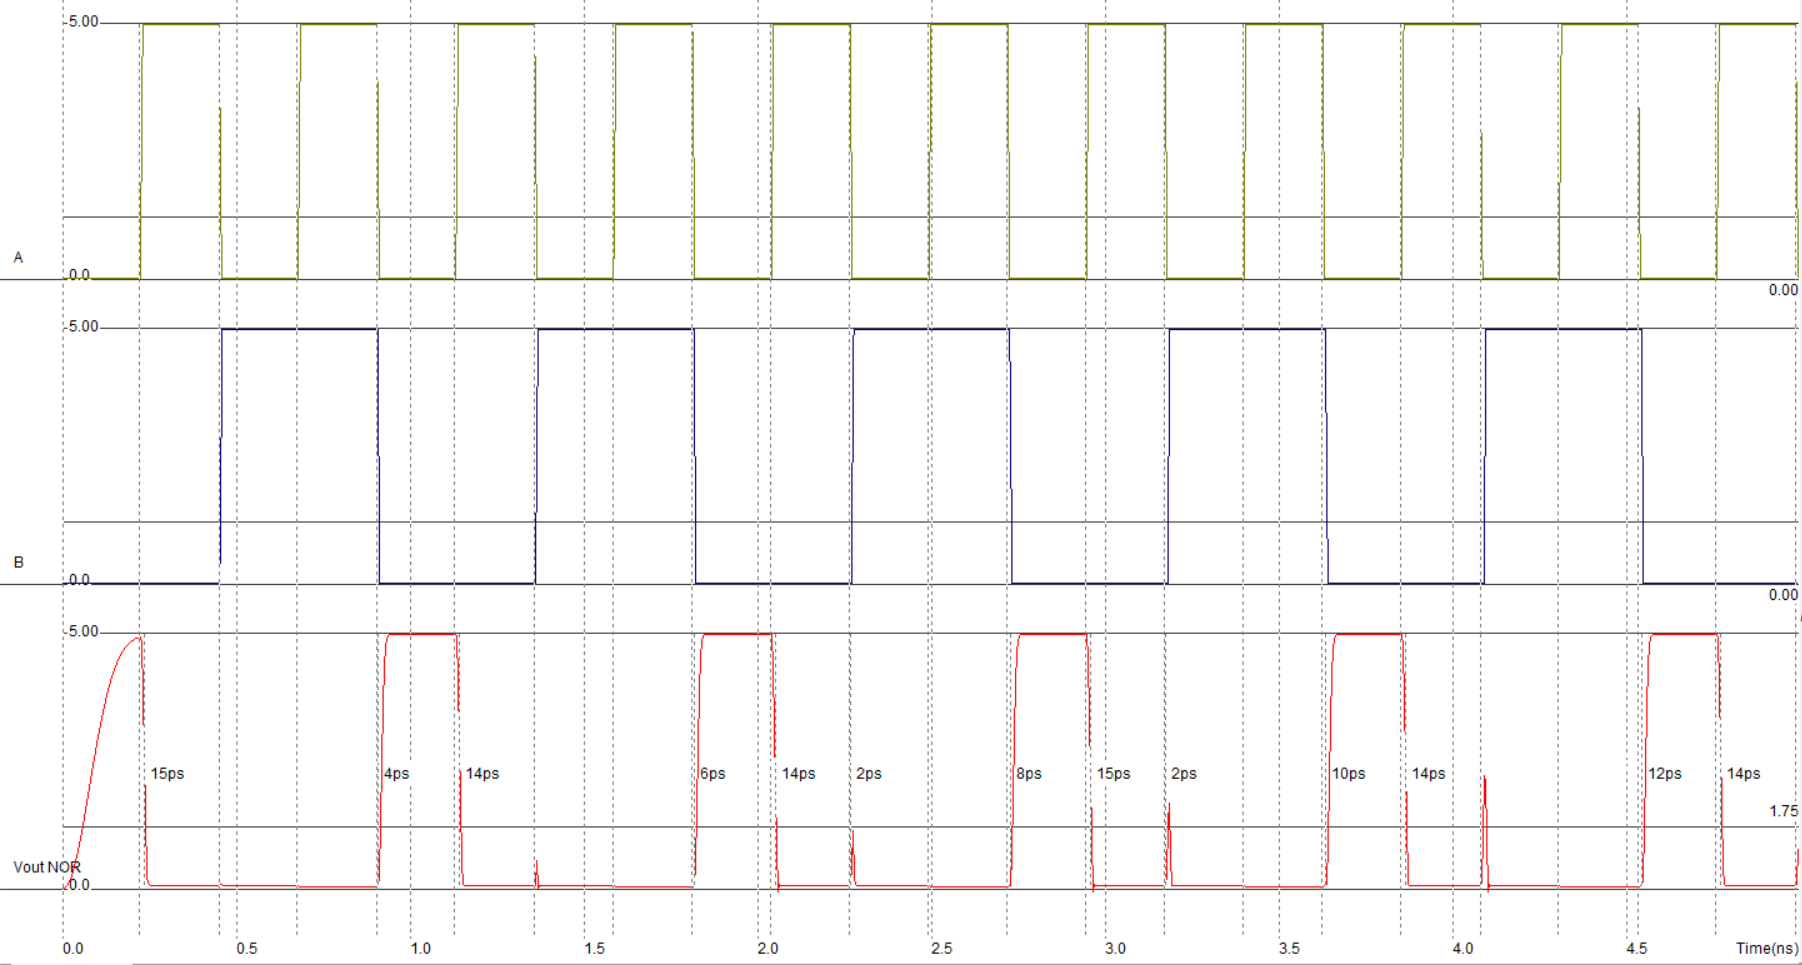
\includegraphics[width=1\linewidth, height=.41\textheight]{Images5/4.1}
		\caption{2 Input NOR-Gate using nMOS Inverter with Resistive Load}
		\label{fig:1}
	\end{figure}
	
	
	
	
	
	\section{Discussion }

	
	The characteristics of 2-input NAND and NOR gates were analyzed using nMOS inverters with resistive and enhancement mode loads. It was observed that for the resistive load configuration, the output voltage improved with an increase in load resistance. This is because a higher load resistance reduces the voltage drop across the resistor, resulting in a higher \( V_{out} \). 
	As the output voltage \( V_{out} \) is given by: $V_{out} = V_{DD} - I_{D} \cdot R$
	

	
	In the enhancement mode load configuration, the output voltage was not perfectly zero. This was due to the finite on-resistance (\( R_{on} \)) of the load transistor, which caused a small voltage drop across the nMOS transistor \( T_1 \). On the other hand, the output voltage was perfectly high, as the load transistor (\( T_2 \)) could fully pull \( V_{out} \) to \( V_{DD} \) without any voltage drop. The simulation results confirmed that both configurations followed the expected logical behavior for the NAND and NOR gates as per their truth tables.
	
	
\end{document}